\subsection{A very basic introduction to networking}
Let's say we have an office in NY. In that office there are end-hosts, such as PCs, server, printers, etc. All of the end hosts need to communicate with each other, for this we introduce a switch, this switch is going to be connected to each of the end-hosts using ethernet cables. A switch is a device with a lot of ports - which are basically slots to connect ethernet cables to - this allows the device to be connected to each other through the switch. The switch is what allows connectivity on my \emph{local area network}. Let's say we add another end-host, a laptop, which is connected wirelessly to the same switch, the laptop will be connected via WIFI to a \emph{wireless access point} and the wireless access point is connected to the switch via an ethernet cable. Now that all the end-hosts are able to communicate, we have built a \emph{local area network}, which means a network that connects devices within the same local area, such as an office or a university campus.


Now that we have built a local area network, we also want these end-hosts to be able to communicate with other devices out on the internet, not just in my local area network. For this we introduce another component, the \emph{router}, which is a device capable of making advanced routing decisions to route traffic between different areas of your network.


Next, now that we have connected the end-hosts to the local are network, and the local area network to the internet via a router. The internet is a very dangerous place, hackers can attack us and other things that we don't want can happen. For security reasons we install a \emph{firewall}, which secures the different parts of our network from each other.


In a larger company we would not just have end-hosts connected to switches connected to routers connected to firewalls connected to the internet. We would have similar local area networks in many other places, for example, we can say that we have a very similar local area network in Boston. The same devices and the same connections. Lets say we want the NY and Boston office to communicate directly without using the internet. We can use a \emph{dedicated connection} between my two routers on both sites for communications to be direct from the NY router to the Boston router, this is called a \emph{wide area network}.


All this is expressed in the next, \emph{network topology diagram}.
\begin{figure}[H]
    \centering
    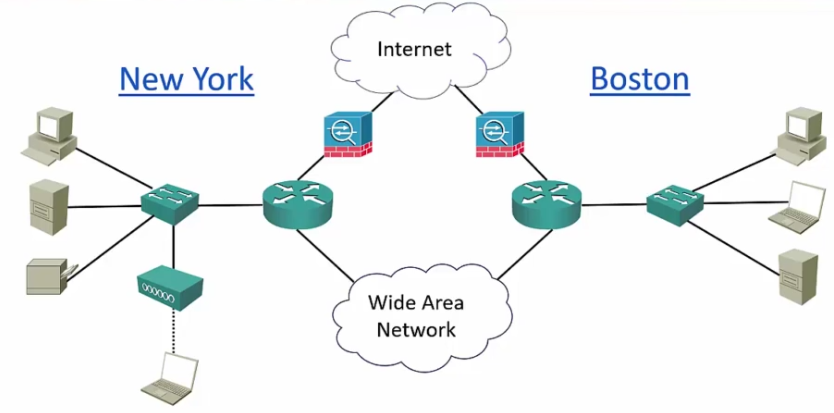
\includegraphics[width=0.4\textwidth]{./Figs/2021-10-10-13-28-12.png}
    % 	\caption{}
\end{figure}

Some other caracteristics of networks are:
\begin{itemize}
    \item Topology: how the devices are connected to the each other.
    \item Speed: the faster, the more cost.
    \item Cost: the monetary cost, effected by the type of devices and technologies used.
    \item Security: all the security features inside and outside the devices.
    \item Availability: making sure that our network always stays up. Mission critical components are typically duplicated, that way we can have an alternative if one were to fail.
    \item Scalability: the topology design lends itself to grow as needed.
    \item Reliability: similar to availability, making sure the network is going to continue to work.
\end{itemize}
    
\section{The OSI Reference model}
\begin{itemize}
    \item The OSI model stands for Open Systems Interconnect model. 
    \item It is standardized by the Organization for Standardization (ISO).
    \item It is a general purpose network that standardizes how computers communicate with one another over a network.
    \item The OSI model is conceptual it is not a physical thing, device, or protocol. It is a concept for humans only, to be able to understand. 
    \item The 7 layer approach to data transmission divides the operations into specific related groups of actions at each layer. A layer serves the layer above it and is served by the layer below it.
\end{itemize}
\subsection{Example}
An example is how you send an email. The sender (the person sending the email) and the receiver (the person receiving the email). 
In the layer 7 - the application layer - which is the layer containing the ``from:'' or the ``to:'' field, this is collected at an application layer. Next the data will be encapsulated by the layer 6 - presentation layer - which deals with the format the data is being handled with. Then the layer 6 information is encapsulated into the layer 5 - session layer - information. That then gets encapsulated to the 4th layer - the transport layer -  which is the layer that specifies what communcation will be used - TCP, UDP, Port number - to prepare it for the next layer. That gets encapsulated into layer 3 - the network layer - which includes the source and destination IP address, a device that operates at layer 3 is the routers. The next the packet is almost being finished, and passed on to the layer 2 - the data link layer - which specifies the mac address - in case we are sending this over an ethernet network -, devices that operate at this layer are switches. Finally the encapsulated and consolidated packet is ready to be sent, this is done in layer 1 - which is the Physical layer - which literally means sending the packet through the wire, a network device that used to be used in this layer are hubs - which are not used anymore -. The email has been sent. The packets travel through the wires and devices to the receiver and the receiver receives packets in the form of electrical signals. 
\begin{figure}[H]
    \centering
    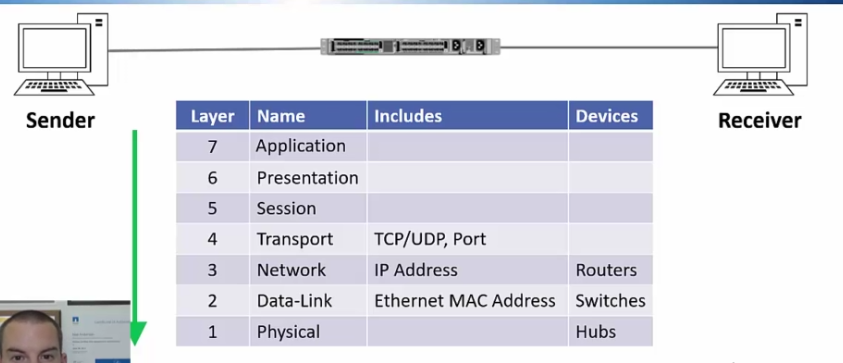
\includegraphics[width=0.4\textwidth]{./Figs/2021-10-10-13-54-03.png}
% 	\caption{}
\end{figure}
The receiver will process the information being received from layer 1 to layer 7, which means that the receiver will grab the data from the first layer and decapsulate it until it has layer 7 data. It comes in at the physical layer, then it it will pass to the data link layer which is 2nd layer, it will perform checks to ensure that the the destination mac address is really for the receiver, if it is not, the receiver will just discard the packet. Next it will look at the layer 3 - which is the network layer - it will check the destination ip address and check if the packet is for it, otherwise it will discard the packet. Then we carry on with the next layer, layer 4 - the transport layer - it will check the port number in which it was received and some other validations. It will continue through the session layer - layer 5 -, the presentation layer - layer 6 -, and the application layer - layer 7 -.
\begin{figure}[H]
    \centering
    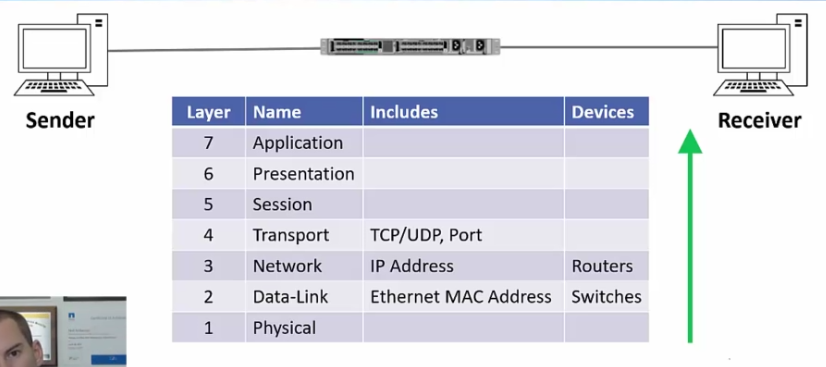
\includegraphics[width=0.4\textwidth]{./Figs/2021-10-10-14-12-16.png}
% 	\caption{}
\end{figure}
Layer 6 and 7 - application and presentation - are considered the upper level, typically used by developers not network engineers. Usually network engineers start to become interested from layer 4 downward.

\subsection{Benefits of the OSI model}
\begin{itemize}
    \item Engineers don't need to design technologies to work end to end from top to bottom of the model. Instead they can just focus on their layer of expertise, and make sure they comply with the standards for the layers above and below.
    \item This leads to open standards and multi-vendor interoperability. 
    \item For example: if you're an application developer, you can just focus on the top three layers, the lower layers are the domain of network engineers. You don't need to understand thzem, you just make sure you are complying with the standards.
    \item Troubleshooting is easier because you can analyse a problem in a logical fashion layer by layer.
    \item It is difficult to convey how important the OSI model is. The OSI model is used to describe problems, solutions, technologies, etcetera. Such as if the cable was disconnected you would say 'it was a layer 1 problem', if you find that the problem was that the user specified a wrong destination - you say - 'it was a layer 7 problem, etcetera.
\end{itemize}

\subsection{OSI Acronyms}
\begin{itemize}
    \item The classic: Please Do Not Throw Sausage Pizza Away.
    \item Network Relevant: Please Don't Need Those Stupid Packets Anyway.
    \item Us relevant: Please Do Not Teach Students Pointless Acronyms.
    \item Useful: Please Do Not Take Sales People's Advice.
    \item Favorite: Please Do Not Touch Superman's Private Area.
\end{itemize}
